% -----------------------------------------------------------------------------
% ########################
% # PREDLOGA ZA POROCILO #
% ########################
%
% @author Matjaz Bevc, Mark Breznik, Amadej Pavsic
% @date   20. december 2020
%
\documentclass[a4paper,12pt]{report}

% -----------------------------------------------------------------------------
% ####################################################
% # UPORABA PAKETOV - NASTAVITEV JEZIKA in KODIRANJA #
% ####################################################
\usepackage[slovene]{babel}
\usepackage[utf8]{inputenc}
\usepackage{lmodern}
\usepackage[T1]{fontenc}
\usepackage[sc]{mathpazo}
\linespread{1.05}
\usepackage[T1]{fontenc}
\usepackage{listings}
\usepackage{pifont}
\usepackage{wasysym}
\usepackage{amssymb}
\usepackage{times}


% -----------------------------------------------------------------------------
% ######################################
% # VNOS KLJUCNIH PARAMETROV BESEDILA  #
% ######################################

\newcommand{\naslov}     {Implementacija modernih spletnih ogrodij - epSHOPmma}
\newcommand{\prviavtor}  {Matjaž Bevc}
\newcommand{\prviindeks} {64180001}
\newcommand{\drugiavtor} {Mark Breznik}
\newcommand{\drugiindeks}{64180002}
\newcommand{\tretjiavtor} {Amadej Pavšič}
\newcommand{\tretjiindeks}{64180022}
\newcommand{\kraj}       {Ljubljana}

% -----------------------------------------------------------------------------
% ###################
% # UPORABA PAKETOV #
% ###################
\usepackage[a4paper,left=25mm,right=25mm,top=20mm,bottom=30mm,includehead]{geometry}

\usepackage{graphicx, epsfig}

\usepackage{fancyhdr}

\usepackage[
colorlinks=true, linkcolor=blue, citecolor=red,
%
pdftitle={\naslov},
pdfauthor={\prviavtor, \drugiavtor},
pdfsubject={Poročilo seminarske naloge pri predmetu Elektronsko Poslovanje},
pdfkeywords={spletna prodajalna, PHP, SSL, MySQL}, a4paper, pagebackref=true, unicode]{hyperref}

% -----------------------------------------------------------------------------
\begin{document}

% -----------------------------------------------------------------------------
% ##################
% # NASLOVNA STRAN #
% ##################
\begin{titlepage}
	\begin{center}
	{UNIVERZA V LJUBLJANI\\[10pt] 
	FAKULTETA ZA RAČUNALNIŠTVO IN INFORMATIKO}

	\vspace{65mm}

	{\Large\textbf{\naslov}}

	\vspace{10mm}

	{\large Poročilo seminarske naloge pri predmetu\\[10pt] Elektronsko poslovanje}

	\vfill
	\vspace{60mm}

\hspace{20mm}
\begin{minipage}[t]{60mm}
	{\bf Študenti}\\
	{\prviavtor} ({\prviindeks})\\ 
	{\drugiavtor} ({\drugiindeks})\\
	{\tretjiavtor} ({\tretjiindeks})
\end{minipage}
%\hfill
\begin{minipage}[t]{50mm}
	{\bf Mentor}\\
	David Jelenc
\end{minipage}
%\hspace{20mm}

	\vspace{25mm}

	{	\kraj, \today}
	\end{center}
\end{titlepage}

% -----------------------------------------------------------------------------
% ##################
% # KAZALO VSEBINE #
% ##################

\tableofcontents

% -----------------------------------------------------------------------------
% ############
% # POVZETEK #
% ############
%\begin{abstract}
%\end{abstract}

% -----------------------------------------------------------------------------
% ##################
% # UVOD DOKUMENTA #
% ##################
\chapter{Uvod}

Pri predmetu EP smo v letu 2020 po navodilih ustvarili spletno trgoino in njej pripadajočo mobilno aplikacijo za Android. Izdelava projekta je v večini slonela na tehnologiji PHP, HTML in SQL. Za shranjevanje podatkov smo uporabili podatkovno bazo MySQL, za katero smo tudi izdelelali scripto .sql, s katero lahko bazo vzpostavimo na poljubnem računalniku. Aplikacija je bila izdelana v razvojnem okolju Android Studio s programskim jezikom Kotlin. 

% -----------------------------------------------------------------------------
% ###################
% # JEDRO DOKUMENTA #
% ###################

% -----------------------------------------------
\chapter{Navedba realiziranih storitev}

V spodnji tabeli je navedena stopnja implementacije posameznih storitev.

\begin{table}[htbp]
\caption{Storitev in stopnja realizacije}
\label{tab1}
\begin{center}
\begin{tabular}{llp{3cm}}
\hline
Naloga & Implementacija \\
\hline
V1 (Captcha) &  \checkmark  \\
V2 (e-mail) & \checkmark \\
V1 (Design) & * - eleganten design, brez asinhrone komunikacije\\
V2 (Slike)& \checkmark \\
V3 (Iskanje)& X -  ni implementirano\\
V4 (Ocene) & \checkmark \\
A1 (Prijava/Odjava) & \checkmark \\
A2 (Profilni podatki) & *  - prikaz podatkov, brez možnosti urejanja \\
A3 (Slike) & \checkmark  \\
A4 (Nakupovanje) & X -  ni implementirano\\
A5 (Kosarica) & X -  ni implementirano \\
A6 (Pretekli nakupi)& \checkmark \\
\hline
\end{tabular}
\end{center}
\end{table}


% -----------------------------------------------
\chapter{Podatkovni model}

Pri izdelavi aplikacije smo v podatkovni bazi SQL ustvarili 6 tabel, od tega tri za uporabnike (stranke, prodajalci, administrator), eno za artikle (vse od imena do slik (v našem primeru longtext formata base64)), eno za narocila in eno povezovalno tabelo naroceniIzdelki za povezovanje naročila z kupljenimi izdelki in njihovo količino - to nam je omogočalo visoko stopnjo fleksibilnosti. Nekaj zanimovsti: atribut activeOrNot nam pove ali je artikel aktiven ali ne, stOcen in sestevekOcen nam omogoča ocenjevanje in povprečno oceno, medtem ko nam eNaslov stranka

\begin{figure}[htb]
	\centering
	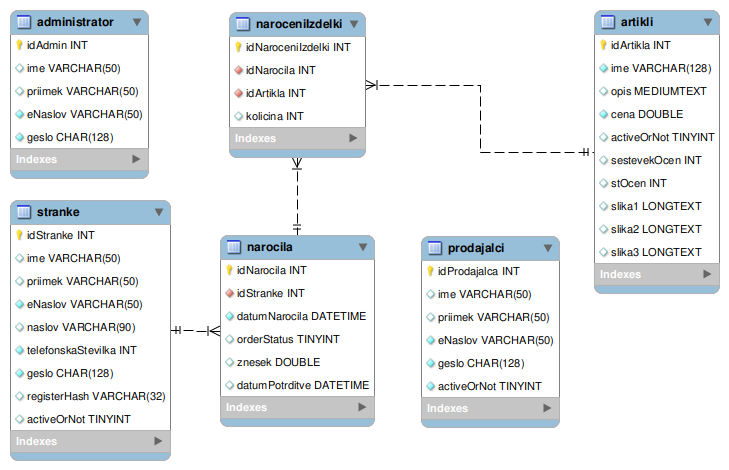
\includegraphics[width=15cm]{sql_baza.png}
	\caption{Logični podatkovni model MySQL}
\label{fig:1}
\end{figure}

% -----------------------------------------------
\chapter{Varnost sistema}

Pri varnosti sitema smo uporabili naslednje tehnike/ protokole:
\begin{table}[htbp]
\caption{Varnost sistema}
\label{tab1}
\begin{center}
\begin{tabular}{llp{3cm}}
\hline
Storitev & Namen \\
\hline
HTTPS &  Omogoča varno komunikacijo med odejemalcem in strežnikom (TLSv1.2)  \\
e-mail potrditev & Preverimo, da ni malomarni račun/ uporabnik/ bot\\
Certificate X.509 & Robusten način za omejitev prijave uporabnikov z višjim nivojem dostopa\\
Filtriranje vnosa& Nazaželeni vnosi - predvsem injekcije kode SQL/ JS/ PHP in napade XSS\\
\hline
\end{tabular}
\end{center}
\end{table}

% -----------------------------------------------
\chapter{Izjava o avtorstvu seminarske naloge}

Spodaj podpisani \textit{\prviavtor} - vpisna številka \textit{\prviindeks}, \textit{\drugiavtor} -  vpisna številka \textit{\drugiindeks} in \textit{\tretjiavtor} -  vpisna številka \textit{\tretjiindeks}, smo soavtorji seminarske naloge z naslovom \textit{\naslov}. S svojimi podpisi zagotavljamo, da smo izdelali ali bili soudeleženi pri izdelavi seminarske naloge.
\newline
\newline
Podpis: {\prviavtor}, l.r. \newline
Podpis: {\drugiavtor}, l.r. \newline
Podpis: {\tretjiavtor}, l.r. \newline



% -----------------------------------------------------------------------------
% #######################
% # ZAKLJUCEK DOKUMENTA #
% #######################
\chapter{Zaključek}

Pri izdelavi seminarske naloge smo se naučili veliko novega, predvsem smo imeli dobro stališče za primerjavo gradnje spletne strani pri EP z PHP in pri SP z Angular, Mongoose, Handlebars in moramo reči, da je uporaba orodij za gradnjo spletnih strani pri predmetu SP, veliko bolj učinkovita kot uporaba  tehnologije kot npr. PHP. Prav tako se nam je zdela uporaba Android aplikacija pri tem predmetu malo nesmiselna, saj bi bilo bolje, da bi se osredotičili le na podatkovno bazo in spletno stran, ne pa da se smo imeli prevelik razpon in se s tem morali posvečati zelo veliko stvarem na enkrat. Ne glede na to verjamemo, da nam bodo na novo pridobljena znanja pri predmetu prišla prav v prihodnosti.
% -----------------------------------------------------------------------------
% ##############
% # LITERATURA #
% ##############
\begin{thebibliography}{99}
\addtocounter{chapter}{1}
\addcontentsline{toc}{chapter}{\protect\numberline{\thechapter}Literatura}
\addtocontents{toc}{\protect\vspace{15pt}}

\bibitem{bib:Enable PHP mail() function on Ubuntu} \emph{Enable PHP mail() function on Ubuntu} (online). 2015. Dostopno na naslovu:
\url{http://researchhubs.com/post/computing/linux-basic/enable-php-mail-function-to-work-on-ubuntu.html}

\bibitem{bib:Store and Retrieve Image from MySQL Database using PHP} CodexWorld. \emph{Store and Retrieve Image from MySQL Database using PHP} (online). 2020. Dostopno na naslovu:
\url{https://www.codexworld.com/store-retrieve-image-from-database-mysql-php/}

\bibitem{bib:How to Implement Email Verification for New Members} Philo Hermans. \emph{How to Implement Email Verification for New Members} (online). 2020. Dostopno na naslovu:
\url{https://code.tutsplus.com/tutorials/how-to-implement-email-verification-for-new-members--net-3824}
\bibitem{bib:Read Owner Cert Data from .p12 file with PHP} Hanzo. \emph{Read Owner Cert Data from .p12 file with PHP} (online). 2016. Dostopno na naslovu:
\url{https://stackoverflow.com/questions/36620108/read-owner-cert-data-from-p12-file-with-php}

\bibitem{bib:Documentation for app developers} Google. \emph{Documentation for app developers} (online). 2020. Dostopno na naslovu:
\url{https://developer.android.com/docs}

\bibitem{bib:Get started with Bootstrap} Bootstrap. \emph{Get started with Bootstrap} (online). 2020. Dostopno na naslovu:
\url{https://getbootstrap.com/docs/4.1/getting-started/introduction/}

\end{thebibliography}

% -----------------------------------------------------------------------------
% ###########
% # DODATEK #
% ###########
\end{document}